\documentclass[11pt,a4paper]{report}
\usepackage{amsmath,amsfonts,amssymb,amsthm,epsfig,epstopdf,url,array,graphicx}
\usepackage[english]{babel}


\theoremstyle{plain}
\newtheorem{thm}{Theorem}[section]
\newtheorem{lem}[thm]{Lemma}
\newtheorem{fact}{Fact}[chapter]
\newtheorem{assm}{Assumption}[chapter]
\newtheorem*{assm*}{Assumption}
\newtheorem{prop}[thm]{Proposition}
\newtheorem*{cor}{Corollary}

\theoremstyle{definition}
\newtheorem{defn}{Definition}[chapter]
\newtheorem{conj}{Conjecture}[section]
\newtheorem{exmp}{Example}[section]

\theoremstyle{remark}
\newtheorem*{rem}{Remark}
\newtheorem*{note}{Note}


\title{Notes on Scalable Blockchain Protocols}
\date{March 14-31, 2015}
\author{Vitalik Buterin}

\begin{document}

\maketitle


\chapter{Introduction}

Currently, all blockchain consensus protocols that are actively in use have a critical limitation: every node in the network must process every transaction. Although this requirement ensures a very strong guarantee of security, making it all but impossible for an attacker even with control over every node participating in the consensus process to convince the network of the validity of an invalid transaction, it comes at a heavy cost: every blockchain protocol that works in this way is forced to choose between a low maximum transaction throughput, and thus at the same time a very high per-transaction cost, and a high degree of centralization.

What might perhaps seem like a natural solution, splitting the relevant data over a thousand blockchains, has the two fundamental problems that it (i) decreases security, to the point where the security of \emph{each individual blockchain} on average does not grow at all as total usage \emph{of the ecosystem} increases, and (ii) massively reduces the potential for interoperability. Other approaches, like merge-mining, seem to have stronger security, though in practice such approaches are either very weak in more subtle ways \cite{mmpetertodd} (and indeed, merge-mined blockchains have successfully been attacked \cite{coiledcoin}) or simply fail to solve scalability, since every merge-miner must process nearly every blockchain.

There are several reasons why scalable blockchain protocols have proven to be such a difficult problem. First, because we lose the guarantee that a node can personally validate every transaction in a block, nodes now necessarily need to employ statistical and economic means in order to make sure that other blocks are secure; in essence, every node can only \emph{fully} keep track of at most a few parts of the entire "state", and must therefore be a "light client", downloading only a small amount of header data and not performing full verification checks, everywhere else. Second, we need to be concerned not only with validity but also with data availability; it is entirely possible for a block to appear that looks valid, and is valid, but for which the auxiliary data is unavailable, leading to a situation where no other validator can effectively validate transactions or produce new blocks since the necessary data is unavailable to them. Finally, transactions must necessarily be processed by different nodes in parallel, and given that it is not possible to parallelize arbitrary computation \cite{parallelcomputing}, we must determine the set of restrictions to a state transition function that will best balance parallelizability and utility.

This paper proposes another set of strategies for achieving scalability, as well as some formalisms that can be used when discussing and comparing scalable blockchain protocols. Generally, the strategies revolve around a "sample-and-fallback" game: in order for any particular block to be valid, require it to be approved by a randomly selected sample of validators, and in case a bad block does come through have a strategy by which a node can provide a proof of malfeasance to the blockchain, reverting the harmful transactions and destroying the malfeasant validators' security deposits in exchange for a reward. Theoretically, under a Byzantine-fault-tolerant model of security, fallback is unnecessary; sampling only is sufficient. However, if we are operating in an anonymous-validator environment, then it is also considered desirable to have a hard economic guarantee of the minimum quantity of funds that needs to be destroyed in order to cause a certain level of damage to the network; in that case, in order to make the economic argument work we use fallback as a sort of incentivizer-of-last-resort, making cooperation the only subgame-perfect equilibrium.

Our basic designs allow for a network consisting solely of nodes bounded by $O(N)$ computational power to process a transaction load of $O(N^{2-\epsilon})$ (we generally use $O(N^\epsilon)$ to denote polylogarithmic terms for simplicity), under both Byzantine-fault-tolerant and economic security models; we then also propose an experimental ``stacking'' strategy for achieving arbitrary scalability guarantees up to a maximum of $O(exp(N/k))$ transactional load, although we recommend that for simplicity implementers attempt to perfect the $O(N^{2-\epsilon})$ designs first.

\chapter{Definitions}

\begin{defn}[State]
A \emph{state} is a set of data.
\end{defn}

\begin{defn}[Transaction]
A \emph{transaction} is a set of data. A transaction typically includes a cryptographic signature from which one can verify its sender, though in this paper we use "transaction" in some contexts more generally.
\end{defn}

\begin{defn}[State Transition Function]
A \emph{state transition function} is a function $APPLY(\sigma, \tau) \rightarrow \sigma \cup \{\varnothing\}$, where $\sigma$ and $\sigma'$ are states and $\tau$ is a transaction. If $APPLY(\sigma, \tau) = \varnothing$, we consider $\tau$ \emph{invalid in the context of $\sigma$}. A \emph{safe state transition function} $SAFE(APPLY) = APPLY'$ is defined by $APPLY'(\sigma, \tau) = \{\sigma \; if \; APPLY(\sigma, \tau) = \varnothing \; else \; APPLY(\sigma, \tau)\}$.
\end{defn}

For simplicity, we use the following notation:

\begin{itemize}
\item
$APPLY(\sigma, \tau) \rightarrow \sigma'$ becomes $\sigma + \tau = \sigma'$
\item
$SAFE(APPLY)(\sigma, \tau) \rightarrow \sigma'$ becomes $\sigma {++} \tau = \sigma'$
\item  
Given an ordered list $T = [\tau_1, \tau_2, \tau_3...]$ and a state $\sigma$, we define $\sigma + T = \sigma + \tau_1 + \tau_2 + ...$
\item
Given an ordered list $T = [\tau_1, \tau_2, \tau_3...]$ and a state $\sigma$, we define $\sigma_0 = \sigma$ and $\sigma_{i+1} = \sigma_i ++ \tau_{i+1}$. We denote with $T \setminus \sigma$ the ordered list of all $\tau_i \in T$ such that $\sigma_i + \tau_i \ne \varnothing$.
\item
T is \emph{valid in the context of $\sigma$} if $T = T \setminus \sigma$
\item
$[n]$ is the set $\{1, 2, 3..... n\}$
\end{itemize}

\begin{defn}[Replay-immunity]
A state transition function is \emph{replay-immune} if, for any $\sigma$, $\tau$ and $T$, $\sigma + \tau + T + \tau = \varnothing$. Generally, we assume that all state transition functions used in consensus protocols are replay-immune; otherwise, the protocol is almost certainly vulnerable to either exploits or denial of service attacks.
\end{defn}

\begin{note}
Replay-immunity is \emph{not} a sufficient condition for being double-spend-proof.
\end{note}

\begin{defn}[Commutativity]
Two transactions or lists of transactions $T_1$, $T_2$ are \emph{commutative in the context of $\sigma$} if $\sigma + T_1 + T_2 = \sigma + T_2 + T_1$.
\end{defn}

\begin{defn}[Compatibility]
Two transactions or lists of transactions $T_1$, $T_2$ are \emph{compatible in the context of $\sigma$} if $\sigma + T_1 + T_2 = \varnothing$ and $\sigma + T_2 + T_1 = \varnothing$ if and only if either $\sigma + T_1 = \varnothing$ or $\sigma + T_2 = \varnothing$.
\end{defn}

\begin{defn}[Partitioning scheme]
A \emph{partitioning scheme} is a bijective function $P$ which maps possible values of $\sigma$ to a tuple $(\sigma_1, \sigma_2 ... \sigma_n)$ for a fixed $n$. For simplicity, we use $\sigma[i] = P(\sigma)[i]$, and if S is a set, $\sigma[S] = \{i: P(\sigma)[i] \; for \; i \in S\}$. An individual value $\sigma[i]$ will be called a \emph{subspace}, and a value $i$ will be called a \emph{subspace index}.
\end{defn}

\begin{defn}[Affected area]
The \emph{affected area} of a transaction (or transaction list) $\tau$ in the context of $\sigma$ (denoted $AFFECTED(\sigma, \tau)$) is the set of indices $S$ such that $(\sigma + \tau)[i] \ne \sigma[i]$ for $i \in S$ and $(\sigma + \tau)[i] = \sigma[i]$ for $i \notin S$.
\end{defn}

\begin{defn}[Observed area]
The \emph{observed area} of a transaction (or transaction list) $\tau$ in the context of $\sigma$ (denoted $OBSERVED(\sigma, \tau)$) is the set of indices $S$ such that for every $i \in S$, either $i \in AFFECTED(\sigma, \tau)$, or there exist two different potential values of $a$, $b$, such that if we define $\psi_a$ to be equal to $\sigma$ except with $\psi_a[i] = a$ and similarly $\psi_b$ equal to $\sigma$ except with $\psi_b[i] = b$, then $(\psi_a + \tau)[j] \ne (\psi_b + \tau)[j]$ for some $j \in AFFECTED(\sigma, \tau)$.
\end{defn}

\begin{note}
The observed area of a transaction, as defined above, is a superset of the affected area of the transaction.
\end{note}

\begin{thm}
If, in the context of $\sigma$, the observed area of $T_1$ is disjoint from the affected area of $T_2$ and vice versa, then $T_1$ and $T_2$ are commutative and compatible.
\end{thm}

\begin{proof}
Suppose a partition of $[n]$ into the subsets $a = AFFECTED(\sigma, T_1)$, $b = AFFECTED(\sigma, T_2)$ and $c = [n] \setminus a \setminus b$. Let us repartition $\sigma$ as $(\alpha, \beta, \gamma)$ for $\sigma[a]$, $\sigma[b]$ and $\sigma[c]$ respectively. Suppose that $\sigma + T_1 = (\alpha', \beta, \gamma)$, and $\sigma + T_2 = (\alpha, \beta', \gamma)$. Because $a$ is outside the observed area of $T_2$ (as it is the affected area of $T_1$), we can deduce from the previous statement that $(x, \beta, \gamma) + T_2 = (x, \beta', \gamma)$. Hence, $\sigma + T_1 + T_2 = (\alpha', \beta, \gamma) + T_2 = (\alpha', \beta', \gamma)$. Similarly, because $b$ is outside the observed area of $T_1$, $\sigma + T_2 + T_1 = (\alpha, \beta', \gamma) + T_1 = (\alpha', \beta', \gamma)$.
\end{proof}

\begin{note}
The observed areas of $T_1$ and $T_2$ are allowed to intersect! However, in the rest of this paper we will follow a fairly dumb rule of focusing on disjointness of observed areas as the primary criterion of disjointness for the sake of simplicity, and we will leave it as an exercise to the reader to determine whether one can improve the protocols' versatility without compromising safety by making a finer distinction.
\end{note}

\begin{defn}[Disjointness]
Two transactions are \emph{disjoint} if there exists a partition such that the observed area of each transaction is disjoint from the affected area of the other. If two transactions are disjoint then, as shown above, they are commutative and compatible.
\end{defn}

\begin{defn}[Effectiveness]
The \emph{effectiveness} of a partitioning scheme is the extent to which it manages to split transactions up into sets which are pairwise disjoint.
\end{defn}

\begin{note}
Highly effective partitioning schemes in practice will likely have to be adaptive, changing over time to capture disjoint sets of transactions. However, one disadvantage of such adaptivity, if not implemented carefully, is that it leads to unpredictable gas pricing in the context of state transition functions that try to meter the difficulty of processing a transaction and charge fees to the sender or participating accounts based on that cost metric.
\end{note}

\begin{defn}[Block]
A \emph{block} is a data packet, encoding a collection of transactions typically alongside verification data, a pointer to the previous block, and other miscellaneous metadata. There typically exists a \emph{block-level state transition function} $APPLY$, where $APPLY(\sigma, \beta) = \sigma + T$, where $T$ is a list of transactions. We of course denote $APPLY(\sigma, \beta)$ with $\sigma + \beta$. A block is valid if $T$ is valid in its respective contexts, and if it satisfies other validity criteria that may be specified by the protocol. In many protocols, there exists a special ``block finalization function''; we model this by saying that we have a rule that every block is allowed to include a ``virtual transaction'' that effects the desired state transition.
\end{defn}

\begin{defn}[Proposer]
The \emph{proposer} of a block is the user that produced the block.
\end{defn}

\begin{defn}[Validators]
The \emph{validators} in a cryptoeconomic state machine are the users that are involved in the consensus process of agreeing on blocks.
\end{defn}

\begin{defn}[Blockchain]
A \emph{blockchain} is a tuple $(G, B)$ where $G$ is a \emph{genesis state} and $B$ is an ordered list of blocks. Cryptographic references (ie. hashes) are typically used to maintain the integrity of a blockchain and allow it to be securely represented only by its final block. A blockchain is valid if $B \setminus G = B$ (ie. all blocks are valid in their respective contexts if applied to $G$ sequentially). 
\end{defn}

\begin{defn}[Parent]
The \emph{parent} of a state $\sigma$ is defined as the state $\sigma_{-1}$ such that $\sigma_{-1} + \beta = \sigma$ for some $\beta$. For genesis states, we define $PARENT(\sigma) = \varnothing$.
\end{defn}

\begin{defn}[Ancestor]
The set of \emph{ancestors} of a state $\sigma$ is recursively defined via $ANC(\sigma) = \emptyset \; if \; PARENT(\sigma) = \varnothing \; else \; \{PARENT(\sigma)\} \cup ANC(PARENT(\sigma))$.
\end{defn}

\begin{defn}[Weight function]
A \emph{weight function} is a function $W(u, \sigma)$ on the set of users $u_1 ... u_n$ (each of which is assumed to have a private and public key) in the context of a state $\sigma$, such that for all users in the network, $\sum_{i=0}^n W(u_i, \sigma) = 1$. ``$k$ of all weight'' will be used to denote the idea of a subset of users such that the sum of their weights is $k$. 
\end{defn}

\begin{note}
A combination of a weighting function and a threshold $0.5 < t < 1$ produces a quorum system.
\end{note}

\begin{defn}[State root function]
A \emph{state root function} is a collision-proof preimage-proof function $R(\sigma) \rightarrow x \in \{0, 1\}^k$ for some small $k$ (usually $k = 256$). $R$ can also be applied to subspaces.
\end{defn}

\begin{defn}[Partition-friendliness]
A state root function is partition-friendly with respect to a particular partitioning scheme if one can compute $R(\sigma)$ by knowing only $R(\sigma[0]), R(\sigma[1]) ... R(\sigma[n])$. 
\end{defn}

\begin{assm}
Any state root function that will be used by any of the protocols described below will be partition-friendly with respect to any partitioning scheme that will be used by the protocols.
\end{assm}

\begin{defn}[Availability]
A state σ is \emph{available} if, for every $i \in [n]$, $\sigma[i]$ can be readily accessed from the network if needed.
\end{defn}

\begin{defn}[Altruist]
An altruist is a user that is willing to faithfully follow the protocol even if they have an opportunity to earn a profit or save on computational expenses by violating it. However, we do not assume that altruists are willing to voluntarily incur losses (as opposed to forgoing gains) if the protocol demands it.
\end{defn}

\begin{note}
This asymmetry roughly captures the standard behavioral-economics understanding of altruism in humans; we are fine with not stealing, but don't really donate all that much to charity.
\end{note}

\begin{assm}
There exists some weight function $W_A$ such that there exists a constant $0 < l < \frac{1}{3}$ such that at least $l$ of weight is altruistic.
\end{assm}

\begin{lem}
A sufficient condition of availabilty is for every $\sigma[i]$ to be in the hands of at least one altruist.
\end{lem}

\begin{proof}
An altruist will be willing to provide data to anyone who asks because that is what the protocol asks them to do.
\end{proof}

\begin{note}
Even if data is available, we do need to make sure in practice that individual data providers will not have their computational capacity overwhelmed. Typically, we make the assumption that the average quantity of nodes that are interested in a particular substate is limited (though some substates can certainly grow to be much more popular than others).
\end{note}

\begin{defn}[Cryptoeconomic State Machine]
A \emph{cryptoeconomic state machine} is a tuple $(G, APPLY, P, F)$ where $G$ is a \emph{genesis state}, $APPLY$ is a state transition function and $P$ is a process for determining the next block. The cryptoeconomic state machine maintains a ``current state'' $\sigma$, repeatedly employs $P$ (by incentivizing validators to carry out their individual roles in P) in order to determine a ``next block'' $\beta$, and then sets $\sigma \leftarrow \sigma + \beta$. $F$ is a process which can be used by a user to determine a recent value of $\sigma$. Desired properties for a cryptoeconomic state machine are:

\begin{itemize}
\item
\emph{Consistency}: everyone sees the same value of $\sigma$ for maximally recent iterations of $P$. If $\sigma$ is too large for any user to download in its entirety, we understand this to mean that everyone sees the same value of $R(\sigma)$.
\item
\emph{Data availability}: all of $\sigma$ is available.
\item
\emph{Non-reversion}: $\sigma$ ideally only changes through the application of additional blocks; it should not revert to previous values. If it does sometimes revert to previous values, the total number and depth of transactions ``undone'' during such a revert should be minimized.
\item
\emph{Validity}: $\sigma$ only ever attains values that are the result of $G + T$ for some transaction list $T$, where $T$ can be produced, using the set of all data that has ever been produced by any user as input, in polynomial time. That is, ``illegal transitions'' that cannot be explained by one or more transactions do not occur.
\item
\emph{Byzantine fault-tolerance}: the above guarantees remain even if up to $k$ of all weight (eg. $k = \frac{1}{3}$) fails to follow the protocol and/or misbehaves arbitrarily (including irrationally).
\item
\emph{Economic security}: the above guarantees survive even if all users except altruists are rational, and are being bribed by an attacker with a budget less than $b * L$ where $b$ is a constant and $L$ is some metric of the value of economic activity in the system.
\item
\emph{Complete security}: the guarantee of economic security survives even if up to $k$ of all weight misbehaves arbitrarily (including irrationally).
\end{itemize}
\end{defn}

\begin{note}
The definition of economic security used above is taken from Vlad Zamfir's model of a ``bribing attacker'' \cite{zamfir}. Bribes do not need to represent literal monetary or other bribes; they can represent blackmail, threats, governmental influence, and even arbitrary personal tastes and prejudices; the intent is to model incentives outside the system by making the assumption that the size of these incentives is bounded by $b * L$. Complete security (ie. economic security under Byzantine faults), rather than simply economic security, is required because, in practice, there do also exist validators that are so irrational that they would pass on even a trillion-dollar incentive in order to stray from the protocol in some way, and it is sometimes possible to inflict extremely high disincentives against specific agents at only medium cost, eg. by means of violence.
\end{note}

\begin{assm}
The ``economic metric of activity'' used to define economic security, transaction load, and the number of users are all proportional to each other.
\end{assm}

\begin{defn}[Scalability]
A cryptoeconomic state machine is \emph{scalable} if, assuming each individual user has computational power, storage and bandwidth bounded above by $N$, the state machine can process $\omega(N)$ (ie. strictly greater than $O(N)$) transactions (with combined Kolmogorov complexity $\omega(N)$) and operate on states of size and Kolmogorov complexity $\omega(N)$.
\end{defn}

\begin{lem}
It is not possible to achieve scalability for arbitrary state transition functions.
\end{lem}
\begin{proof}
Suppose the state transition function $\sigma + \tau = H(\sigma + \tau)$ for some hash function. This is clearly unparallelizable. Hence, the transaction rate is bounded above by the serial computational power of one node.
\end{proof}

\begin{lem}
It is not possible to achieve guarantees of scalability and data availability with greater than $\frac{1}{2}$ Byzantine fault tolerance for many state transition functions under any weight function $W$.
\end{lem}

\begin{note}
First, we should see that there do exist state transition functions for which a complete guarantee of data availability is compossible with scalability: at the least, the function where $\sigma + \tau = \sigma$ for all $\tau$. So the functions for which such a guarantee is impossible will need to be more complex. We will focus on the case where each transaction modifies at least $d$ independent bits of entropy to the state (ie. a diff of the state produced by $t_1 ... t_n$ will have Kolmogorov complexity at least $dn$).
\end{note}

\begin{proof}
The user themselves can verify at most $O(N)$ bits of the file, so there is still $\omega(N)$ entropy that the user must validate is available. Note that it must be possible to prove availability with only the participation of $\frac{1}{2}$ of the weight; otherwise $\frac{1}{2}$ of the weight disappearing will prevent any successful blocks. Now, we need to prove that $\frac{1}{2}$ of the weight under $W$ will at least sometimes be less than $1 - l$ of the weight under $W_A$ (the function under which we are assuming that we have $l$ weight of altruists). Suppose that is not the case. Then, split up the nodes into disjoint sets $S_1$ and $S_2$, such that each $S_i$ has less than $\frac{1}{2}$ weight under $W$. Then, each set will have weight at least $1 - l$, and so the combined set will have weight $2 - 2l > 1$. Hence, it is possible for an attacker with $\frac{1}{2} < k < 1 - l$ of weight under $V$ to either convince at least some users that a block with actually unavailable data has available data, or shut down the network.
\end{proof}

\chapter{Cryptographic and Cryptoeconomic Primitives}

\begin{defn}[Sampling function]
A \emph{sampling function} is a function $SAMPLE(W, k, m) \rightarrow {u_1 ... u_m}$ that takes a weight function $W$, a salt $k$ and a number $m$ and outputs a pseudorandomly selected (weighted by $W$) sample of $m$ users.
\end{defn}

\begin{exmp}
Arrange all users $u_1 ... u_n$ in order of public key, and assign the range $[\sum_{i=1}^{j-1} W(u_i)...\sum_{i=1}^j W(u_i)]$ to user $u_j$ for all $1 <= j <= n$. For all $1 \le h \le m$, return the user whose range includes the value $\frac{H(k + h)}{2^{256}}$ for some hash function $H$.
\end{exmp}

\begin{defn}[Merkle tree protocol]
A \emph{Merkle tree protocol} is a scheme consisting of two functions:
\begin{itemize}
\item
$P(\sigma, i) \rightarrow \pi$
\item
$V(\rho, i, \pi, V) \rightarrow \{0, 1\}$
\end{itemize}
$V$ should only return 1 if $\pi$ is a proof showing that $V = \sigma[i]$ for some $\sigma$ such that $R(\sigma) = \rho$.
\end{defn}

\begin{note}
There exist Merkle tree protocols for which $P$ and $V$ can be computed in logarithmic time \cite{merkle}, and there exist state root functions which can determine the new state root after a minor change to a value or even the introduction or removal of a partition in logarithmic time.
\end{note}

\begin{defn}[Merkle branch]
A \emph{Merkle branch} is the tuple $(V, \pi)$.
\end{defn}

\begin{defn}[Proof of custody]
A \emph{proof of custody} protocol \cite{zamfirpoc} is a tuple of three functions, $M$, $P$ and $V$, where:

\begin{itemize}
\item
$M(F) \rightarrow \{0,1\}^k$, usually with $k = 256$, maps a file to a specialized root hash.
\item
$P(F, k) \rightarrow \pi$ produces a proof from a file and a key.
\item
$V(M, K, \pi) \rightarrow \{0,1\}$ verifies the proof.
\end{itemize}

It should only be possible to produce a proof $\pi$ that satisfies $V$ if one simultaneously has (i) the file, and (ii) the private key $k$ whose associated public key is $K$.
\end{defn}

\begin{note}
There exist naive algorithms for computing $M$ and $P$ in $O(N^2)$ time, and more sophisticated algorithms that achieve $O(N^{1+\epsilon})$ time \cite{ffterasurecode}. Proofs are logarithmically sized and $V$ can be computed in logarithmic time.
\end{note}

\begin{defn}[Cryptoeconomically secure entropy source]
A cryptoeconomically secure entropy source is a protocol inside of a state transition function that regularly generates fixed-size values such that, for any predicate $P$ which the next value would normally have with probability $p$ assuming everyone honestly follows the protocol, the cost of making the value have that predicate with probability $p' > p$ is bounded below by $b * (p' - p)$ multiplied by some economic metric of activity in the state machine for some constant $b$ (independent of $P$).
\end{defn}

\begin{exmp}
The cryptoeconomically secure entropy source used in NXT\cite{nxtinside} is defined recursively as follows:
\begin{itemize}
\item
$E(G) = 0$
\item 
$E(\sigma + \beta) = sha256(E(\sigma) + V(\beta))$ where $V(\beta)$ is the block proposer of $\beta$.
\end{itemize}
The only way to manipulate the result is for the block proposer to disappear, leading to another proposer taking over. However, this action is costly for the proposer as the proposer loses a block reward. Note that the optimal strategy is to disappear with probability $0 < q <= 1$ only when the predicate will be unsatisfied with the proposer participating but will be satisfied with the next proposer partipating; if a predicate has probability $p$ this entails disappearing $p * (1-p) * q$ of the time, meaning that the predicate will be satisfied $p + p * (1-p) * q$ of the time instead of $p$ of the time, a probability increment of $p * (1-p) * q$ at the cost of $p * (1-p) * q * R$ if $R$ is the signing reward. Hence, the cost-to-influence ratio $b$ is exactly equal to $R$.
\end{exmp}

\begin{defn}[zk-SNARK scheme]
A zk-SNARK scheme is a tuple of three functions $G$, $P$, $V$, where:
\begin{itemize}
\item
$G(prog) \rightarrow k$ generates a "verification key" from a program.
\item
$P(prog, I_s, I_p) \rightarrow \pi$ generates a proof that $prog(I_s, I_p)$ for some secret inputs $I_s$ and public inputs $I_p$ is equal to its actual output, $o$.
\item
$V(k, I_p, o, \pi) \rightarrow \{0, 1\}$ verifies a proof, accepting it only if $\pi$ is actually a proof that $prog(I_s, I_p) = o$ where $G(prog) = k$.
\end{itemize}
Additionally, $\pi$ should reveal no information about the value of $I_s$. Schemes exist \cite{snark} to perform $G$ and $P$ in a time equal to $O(N*log^k(N))$ for a small $k$ where $N$ is the number of execution steps, and $V$ can be computed in some cases in polylogarithmic time and in some cases in constant time.
\end{defn}

\begin{note}
We provide algorithms which achieve scalability without zk-SNARKs, however we will show how zk-SNARKs can also be used in scalable blockchain protocols. Particularly, note that zk-SNARKs may be usable as a form of proof of custody.
\end{note}

\begin{defn}[Decentralized oracle scheme]
A decentralized oracle scheme is a mechanism which asks a set of participants to provide an answer to a subjective question (eg. "what was the temperature in San Francisco on 2015 Jan 9?"), and attempts to incentivize the participants to answer correctly. The output of the mechanism is generally considered to be the majority answer, and as input the scheme usually requires an economic subsidy.
\end{defn}

\begin{exmp}
A simple decentralized oracle scheme, called ``SchellingCoin'', has the following rules:
\begin{itemize}
\item
Each of $N$ participants must vote either $1$ or $0$ on a question (a scalar-valued or multi-valued question is modeled as a series of binary questions).
\item
A participant whose vote aligns with the majority vote receives a reward of $P$.
\item
A participant whose vote does not align with the majority vote receives a reward of $0$.
\end{itemize}
SchellingCoin is vulnerable to zero-cost equilibrium flips, and so under a formal definition of economic security it cannot be viewed as having any security margin at all, though in practice it is likely to work reasonably well due to the difficulty of coordination problems. An attacker with a budget greater than $P$ and the ability to credibly commit to to providing a bribe under certain conditions in the future can, assuming rationality of the participants, effect an equilibrium flip toward a wrong answer at no cost \cite{pepsilon}.

More advanced versions of Schelling-coin include a version augmented with Sztorcian counter-coordination \cite{sztorc}, which massively increases the size of the economic incentive required to effect an equilibrium flip, and a version in which substantial disagreements lead to the blockchain simply forking, leaving users to choose which version they follow (the economic argument is that users will prefer the version which contains more honest voters, and users that don't have access to the subjective information about the specific fact in question can figure out which version is ``correct'' by looking at the market price of the tokens associated with each version). 
\end{exmp}

\chapter{A Byzantine-fault-tolerant Scalable Consensus Algorithm}

Suppose a construction where the state is partitioned into $n = O(N^{1-\epsilon})$ sections (``substates''), and each substate is itself partitioned into very small parts (eg. one per account). We define three ``levels'' of objects:

\begin{itemize}
\item
A \emph{super-block} is a block in the top-level consensus process. The \emph{header chain} is the blockchain of super-blocks.
\item
A \emph{block} is a package containing:

    \begin{itemize}
    \item
    $T$, a list of transactions
    \item
    $D$, the set of Merkle branches for the observed area of T on the fine-grained sub-partition level, ie. where the value proven by each Merkle branch is only constant-size (eg. an account)
    \item
    A \emph{header}, consisting of:
        \begin{itemize}
        \item
        $AP$, a map $\{i: R(\sigma[i]) \; for \; i \in OBSERVED(\sigma, T)\}$
        \item
        $AN$, a map $\{i: R(\sigma'[i]) \; for \; i \in OBSERVED(\sigma, T)\}$
        \item
        $S = [s_1 ... s_m]$, an array of signatures
        \item
        $H(T)$
        \item
        $H(D)$
        \end{itemize}
    \end{itemize}
\item
A \emph{transaction} is a transaction as before.
\end{itemize}

We use any non-scalable consensus algorithm (eg. Tendermint) for processing super-blocks, except that we define a custom ``top-level'' state transition function $APPLY'$. As a state, we use $\psi = \{i: R(\sigma[i]) \; for \; i \in [n]\} + E(\sigma) + V(\sigma)$ where $E(\sigma)$ is a cryptoeconomically secure entropy source in $\sigma$ and $V(\sigma)$ is a set of ``validators'' registered in $\sigma$. From the point of view of $APPLY'$, we define a block header $\tau$ as being valid in the context of $\psi$ if the following are all true:

\begin{itemize}
\item
For all $i \in AP$, $\psi[i] = AP[i]$.
\item
For at least $\frac{2m}{3}$ values of $i \in [m]$, $s[i]$ is a valid signature when checked against $SAMPLE(W, E(\sigma) + P, m)[i]$ where $W(\sigma, u_i) = \frac{1}{|V(\sigma)|} \; if \; u_i \in V(\sigma) \; else \; 0$ and $P$ is the public key of the block proposer.
\end{itemize}

If $\tau$ is valid, we set $\psi'$ by:

\begin{itemize}
\item
For all $i \in OBSERVED(\sigma, \tau)$, $\psi'[i] = AN[i]$
\item
For all $i \notin OBSERVED(\sigma, \tau)$, $\psi'[i] = \tau[i]$
\end{itemize}

The block-level state transition function has an additional validity constraint: for the block to be valid, the areas of all $\tau[i]$ must be disjoint from each other.

We do not formally put it into the top-level validation protocol, but we separately state that a validator is only supposed to sign a block if the block meets what we will call \emph{second-level validity criteria} for $\tau$:

\begin{itemize}
\item
Every transaction in $T$ is valid in its context.
\item
$D$, $AP$, and $AN$ are produced correctly.
\end{itemize}

\begin{lem}
Assuming less than $\frac{1}{3}$ of validators are Byzantine, a block that is valid under the above top-level state transition function will produce a top-level state $\psi'$ such that if we define $\sigma'$ with $\sigma' = \{i: R^{-1}(\psi'[i])\}$, $\sigma' = \sigma + T_1 + T_2 + ...$ where $T_i$ is the set of transactions in $\tau_i$.
\end{lem}

\begin{proof}
Suppose that all $\tau_i$ satisfy the second-level validity criteria. Then, note that the observed-but-not-affected area of each $T_i$ remains constant throughout the block, and each substate in the affected area is only modified by one $T_i$, and so we can model the state as a tuple $(O, A_1, A_2, A_3 ... A_n)$ if $\beta$ includes $k$ transactions, where $A_i$ is the affected area of $T_i$ and $O$ is the remaining part of $\sigma$. The state after $T_1$ will be $(O, A'_1, A_2, A_3 ... A_n)$, by disjointness the state after $T_2$ will be $(O, A'_1, A'_2, A_3 ... A_n)$, and so forth until the final state is $(O, A'_1, A'_2, A'_3 ... A'_n)$. If we use the top-level state transition function on $\psi$, we can partition $\psi$ similarly into $(O, B_1, B_2, B_3 ... B_n)$, and a similar progression will take place, with state roots matching up at every step. Hence the final state at this top-level state transition will be made up of the roots of the substaces in $\sigma'$.

Now, suppose that one $\tau_i$ does not satisfy the second-level criteria. Then, validators following the protocol will consider it invalid, and so $\frac{2m}{3}$ validators will not be willing to sign off on it with very high probability, and so the block will not satisfy the top-level criteria.
\end{proof}

Hence, we know that the resulting $\psi'$ will represent a state which is \emph{valid}, in the sense that it can be described as a series of transactions applied to the genesis. This is the validity criterion that we will repeatedly use in order to prove that validity is preserved by other mechanisms that we introduce such as revert mechanics.

Because a sampling scheme is inherently probabilistic, it is theoretically prone to failure, and so we will precisely calculate the probability that the protocol will fail. Assuming a 96-bit security margin, we can consider a probability negligible if the average time between failures is longer than the time it takes for an attacker to make $2^{96}$ computations. If we assume that the cryptoeconomically secure entropy source updates every super-block, and a super-block comes every 20 seconds, then one can reasonably expect a hostile computing cluster to be able to perform $2^{48}$ work within that time, so we will target a failure probability of $2^{-48}$ (this implies roughly one failure per 445979 years of being under attack). We can determine the failure probability with the following formula from combinatorics:
\\
\\
$PE(n, k, p) = p^k * (1-p)^{n-k} * \frac{n!}{k!(n-k)!}$
\\
\\
Where $PE(n, k, p)$ is the probability of an event that occurs with probability $p$ in an attempt will achieve exactly $k$ occurrences out of $n$ attempts. For convenience, we define $PGE(n, k, p) = \sum_{i=k}^n PE(n, i, p)$, ie. the probability of \emph{at least} k occurrences.

We note that $PGE(135, 90, \frac{1}{3}) = 2^{-48.37}$, so 135 nodes will suffice for a $k = \frac{1}{3}$ fault tolerance. If we are willing to lower to $k = \frac{1}{5}$, then $PGE(39, 31, \frac{1}{5}) = 2^{-48.58}$, so 39 nodes will be sufficient. Additionally, note that if we want greater efficiency under normal circumstances, then a bimodal scheme where either 44 out of a particular 50 nodes ($PGE(50, 44, \frac{1}{3}) = 2^{-49.22}$) or 90 out of a particular 135 nodes is a sufficient validity condition will allow the cheaper but equally safe condition to work in the (usual) case where there are almost no malicious nodes, nearly everyone is online and the network is not under attack, and fall back to the more robust but bulkier validation rule under tougher conditions.

\begin{lem}
The above protocol is scalable.
\end{lem}

\begin{proof}
The load of a validator consists of two parts:

\begin{itemize}
\item
validating the header chain
\item
validating the blocks
\end{itemize}

For the header chain, note that the size of each super-block is $n+k_1b+k_2$, where $n$ is the size of the state partition (as each index can be included as an observed area at most once), $b$ is the number of blocks, $k$ is a constant representing the size of $H(T) + H(D) + [s_1 ... s_m]$, and $k_2$ is a constant for miscellaneous super-block data (eg. validators entering and leaving, the entropy source, timestamp, previous block hash). We can require $n \in O(N^{1-\epsilon})$ and $b \le n$ so $b \in O(N^{1-\epsilon})$. One can come up with an algorithm to evaluate the top-level validity of the block in less than $O(N)$ time; the toughest part may be showing that observed areas do not intersect as a set non-intersection algorithm can take $O(k*log(k))$ time for $k$ items and $O(N^{1-\epsilon} * log(N^{1-\epsilon})) < O(N)$, and everythin else should simply take $O(N^{1-\epsilon})$ time.

For block validation, suppose that there are $v \in O(N^{1-\epsilon})$ validators. Each super-block may contain a maximum of $n$ blocks, and $n \in O(N^{1-\epsilon})$. Thus, in total, validators must process at most $m*n$ blocks (as each block must be processed by $m$ validators), and so each validator will on average end up processing $m*m/v \in O(1)$ blocks. If each block has $O(N^{1-\epsilon})$ transactions, then the computational load of this is $m * O(N^{1-\epsilon}) < O(N)$. Hence, the total load of a validator is less than $O(N)$ while the network processes a total of $O(N^{2-\epsilon})$ transactions.

From a bandwidth perspective, the header chain is sent to everyone, but for blocks the block proposer need only send the block to the validators directly, so once again the load per validator is $O(N^{1-\epsilon})$. The only data that a validator needs to verify the block is the observed areas on the sub-partition level, which are provided with proofs inside of $\tau$.
\end{proof}

\chapter{Fallback Schemes}

The previous algorithm provided a guarantee of data availability and validity by simply assuming that at least two thirds of validators are honest. Here, we dispense with that requirement, instead assuming that everyone, except for the $l$ of weight in the hands of altruists and up to $\frac{1}{3}$ of weight in the hands of arbitrarily Byzantine actors, is rational. The first change that we will make is require all validators to provide a security deposit of size $O(N^{1-\epsilon})$ in order to participate in the validation process. By doing this, we have the ability to economically disincentivize actors that we have identified as malfeasant, thereby providing an economic guarantee of security.

If we are trying to achieve scalability through sampling, however, we arrive at a conundrum. Although sampling works well if you assume that a percentage of actors are rational, from an economic standpoint it's not quite so easy. Suppose that there exists an attacker that pre-commits to bribing everyone that falsely provides a signature claiming that a particular block is valid. Then, the attacker would need to make $m$ bribes in order to produce a false block that gets accepted by the network. Becuase the total number of validators is $O(N^{1-\epsilon})$, $m$ validators would only provide a security margin equal to $O(\frac{1}{N^{1-\epsilon}})$ of all economic activity in the system. Hence, there is no fixed bound $b$ of proportionality between the weight and the security margin; the ratio goes lower the larger the system gets.

The solution that we propose is a ``fallback game'': allow any validator to ``challenge'' a particular block's validity by putting some quantity of funds at stake (if no funds are at stake, then an attacker can increase load on the network arbitrarily at no cost), and ask the header chain to be the ``validator-of-last-resort''. If the data for the block is available, then this is easy: the validator provides the full block to the header chain, and the header chain validates the block; if the block is valid, then the challenger loses some portion of their security deposit, and if the block is invalid then the validators that signed the block lose their entire security deposit (and a portion of that deposit goes to the challenger as a reward). The game that arises from this scenario can be seen as follows:

\begin{center}
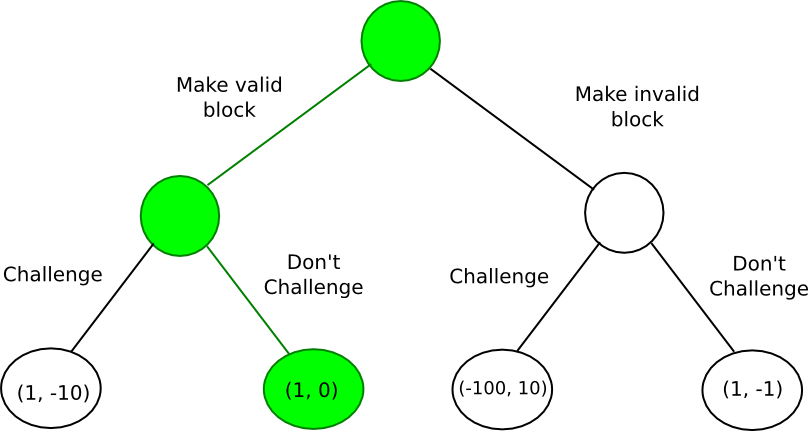
\includegraphics[width=200pt]{game.png}
\end{center}

Above we assume $1$ is the block reward, $-\delta$ is an expected private payoff to the validator of an invalid block getting into the blockchain (all we know about this payoff is that it is less than zero; it could take any magnitude depending on the situation of the particular validator and ultimately does not matter for the purposes of the game-theoretic argument), $100$ is the security deposit, $10$ is the whistleblower's reward and $-10$ is the penalty for whistleblowing falsely (ie. on a valid block). Note that the blockmaker ``plays'' first. If the blockmaker makes an invalid block, then the challenger will challenge, and so the blockmaker will earn $-100$; but by making a valid block the blockmaker will earn $1$. Hence, the blockmaker will make a valid block, and in that case the challenger will earn a higher profit of $0$ rather than $-10$ by not challenging and so will not challenge. Thus providing a valid block is a subgame-perfect equilibrium.

There are two problems with this scheme as described above. The first problem is a technical one: although the scheme remains scalable, Byzantine fault tolerant and economically secure, and even economically secure under a Byzantine failure or Byzantine-fault-tolerant under an economic attack, it is not \emph{scalable under an economic attack}. The reason is that an attacker can spend $\frac{L}{O(\frac{1}{N^{1-\epsilon}})}$ resources by bribing $m$ of the $O(N^{1-\epsilon})$ validators in order to elevate any block to the header level, and so by spending $b * L$ effort the attacker can elevate a total of $O(N^{1-\epsilon})$ blocks. As soon as the size of a block is at least $O(N^{2\epsilon})$ (which happens at $L \in O(N^{1+\epsilon})$), this means that by spending $b * L$ effort the attacker can make the protocol non-scalable.

The solution that we propose is a multi-round escalation game: a challenger proposes a transaction to point out an invalid previous block, and that transaction will be validated by $2m$ validators. If either the challenger or a validator is unhappy with the result, they can then make another challenge, providing twice as high a deposit but resulting in the block being reviewed by $4m$ validators. Another appeal is possible with a 4x deposit, which will be reviewed by $8m$ validators, and so on until all validators participate. Hence, the number of validators which end up being involved in the process is linear in the number of validators bribed. Hence, if the transaction load is $L$ (and so the number of validators is $\frac{L}{O(N^{1-\epsilon})}$), and an attacker spends $b * L$ resources, then the attacker will be able to force a block to be validated by $\frac{b * L}{O(N^{1-\epsilon})}$ validators, ie. a total effort of $O(b * L)$ with per-validator expense $O(\frac{b * L}{O(N^{1-\epsilon})})$, which is less than $O(N)$ for $L < O(N^2)$. Hence, the scheme remains scalable even under economic attack. If one game-theoretically analyzes this game, one finds that the dishonest strategies can be recursively eliminated, making the subgame-perfect equilibrium honesty.

\chapter{Data availability}

The more difficult challenge in going from a statistical Byzantine fault tolerance guarantee to a cryptoeconomic security guarantee comes when the data is not available. Validating data availability through simple cascading fallback is impossible for a simple reason: the attacker can always cheat the system and destroy others' deposits by providing a block with unavailable data at first, waiting for a fallback game to start, and then destroying the security deposits of challengers by suddenly providing the data mid-game.

Additionally, note that unless zk-SNARK protocols are used, if data is not available there is no way to check validity or prove invalidity, and so once challengers get tired of losing security deposits attackers will be able to get invalid blocks included in the blockchain as well (zk-SNARKs in the header may be used to make that attack impossible, but still cannot by themselves prove availability). Hence, what we appear to need is a way of actually cryptographically, and not just cryptoeconomically, proving that data is available at a particular time.

There third four major categories of solutions that we can use. The first is to simply give up on economic security, and rely on the scheme to be secure under a Byzantine-fault-tolerant model. We then ask validators to censor attempts to join the validator pool by parties that appear to be unreliable or likely to be malfeasant. In some cases, particularly regulated financial systems, such restrictions are necessary in any case and so we need to go no further. If we are trying to create a more open network, however, then such a solution is unsatisfactory, and so we arguably need not just Byzantine fault tolerance but also regulation via economic incentives.

The second is to turn the escalating fallback game into a decentralized oracle scheme. Here, we note that the question that we need to vote on during the escalating fallback game is not whether the data \emph{currently is} available, but whether the data \emph{was} available. This is information that can be reasonably expected to be known by most validators, particularly since an attacker taking over $m$ validators is only realistically likely to happen if validators were ``bribed'' (or threatened), and for such a bribe to be effective it would need to be broadcasted to the public. However, it is not information that will be available to absolutely anyone validating the blockchain, particularly in the future. Hence, the ``final round'' of an escalating fallback game (ie. the round where \emph{all} validators participate) is an exactly identical scenario to that faced by decentralized oracle schemes.

There are two approaches to securing decentralized oracle schemes. One is the set of strategies involving Sztorcian counter-coordination, which attempts to naturally set the quantity of funds at stake in proportion to the level of controversy in the question; in the limit, people who do not vote alongside the majority answer lose their entire security deposit. The game-theoretic argument is that if a medium-sized bribe to vote incorrectly is offered, then voters will vote for the correct answer with some of their funds and for the incorrect answer with some of their funds, leading to an equilibrium where the majority of the voting power is still in favor of the correct answer but the users also manage to ``steal'' some of the bribe:

\begin{center}
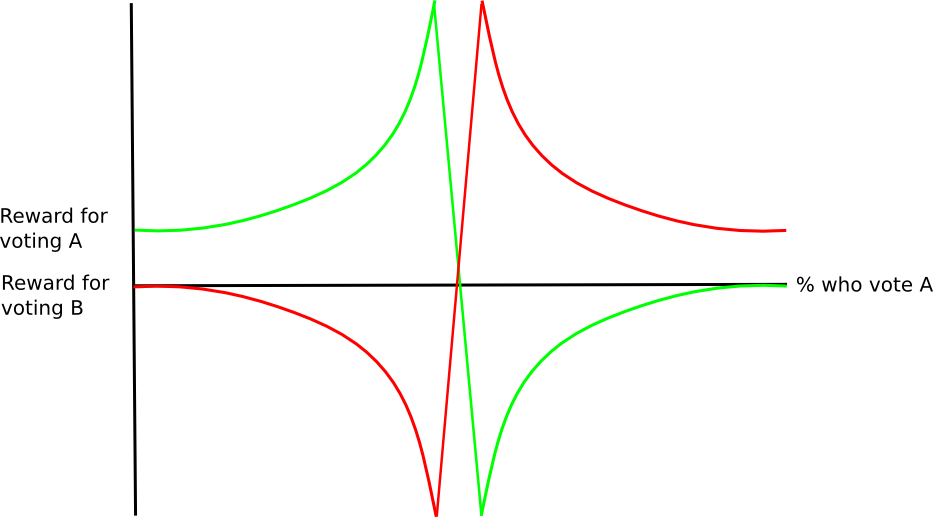
\includegraphics[width=165pt]{schellingcoin_payoff1.png}
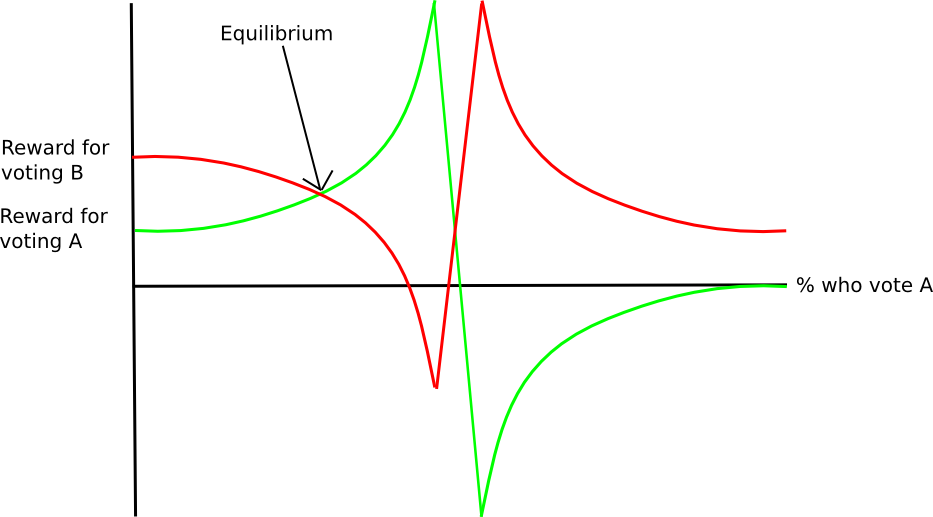
\includegraphics[width=165pt]{schellingcoin_payoff2.png}
\end{center}


This approach accepts that attackers with a budget even larger than the size of everyone's security deposits will be able to cause everyone to flip to voting incorrectly as an equilibrium, but advocates note that attackers that large will also be able to arbitrarily disrupt the underlying blockchain consensus anyway.

The second approach is to fall back to ``subjective resolution'': if, during the last round, the majority of voters vote incorrectly, then we consider that super-block to be invalid, and the community simply coordinates on a fork to a version of the header chain which contains the honest validators. On the interface level, this would be done by making it very easy for users to switch to a different fork on their client, ideally by simply putting in a hash. This reliance on human judgement at the last level makes the difficulty of an ``equilibrium flip'' essentially infinite, instead requiring the attacker to bribe everyone outright, but because the process only happens at the last step of a fallback game under normal circumstances users will not be bothered by the need to make any manual fork swiches at all; like nuclear deterrence, the point of the scheme is to threaten to be used, not to actually be used. In either case, however, one can see that an attacker that can overcome the final-round vote will also be able to overcome the underlying non-scalable blockchain consensus at equal cost, and so scalability does not introduce additional risks.

A third category of solution, one which avoids final-subjective-resolution but at the cost of other questionable assumptions and substantial efficiency loss, is proof of custody. Using a proof of custody scheme, we require $\frac{2}{3}$ of the sample validating a block to make a proof that they \emph{actually have} the validation data - or, more precisely, that the same computer simultaneously holds (i) the validation data, and (ii) the private key of that validator. If a validator notices that a block for which data was unavailable went into the header chain, but for which the proofs of custody appear valid, then we cryptographically know that there exists \emph{some} piece of data which the proofs of custody represent. Hence, if a validator submits a challenge, we know that at least one altruist will provide that data, at which point a larger consensus group will be able to check validity.

However, here we have a problem: what if, instead of bribing validators to vote on an invalid or unavailable block and thus losing their security deposits, the attacker simply bribes validators to give the attacker their keys? In this case, the attacker actually will be able to provide proofs of custody without anyone else seeing the data, since the attacker has all the keys, and so the proof of custody appears ineffective. Here, we can make a case that the scheme is still effective, but the case will be an imperfect one and in many ways lacking the standards of a formal proof.

We can set up a game where any user can with a short delay (eg. 1h) recover the funds from a security deposit to a different address, sacrificing at least $\frac{2}{3}$ of the funds in the process. During the window, a keyholder can ``outbid'' the previous recovery attempt with a new attempt that offers to sacrifice more and keep less. Given this scheme, if there arises a situation where there are two keyholders, a Bertrand competition argument ensures that the final value of the deposit is roughly equal to one transaction fee (if the attacker tries to get around this by having reputation, then an altruist keyholder can wait until the deposit expires, withdraw the funds, and blame the attacker).

Thus users, particularly the altruists, will have no problem risking their deposits by putting up a challenge, and so the only thing that the attacker will be able to do through the bribe attack is increase load on the validators.

Ultimately, note that all of the above arguments are highly theoretical, and perhaps introducing complex solutions to deal with them is not necessary, particularly if it comes at the cost of highly expensive proof-of-custody schemes. Thus, we recommend the final-subjective-resolution approach due to its simplicity.

\chapter{Reverting}

One important issue that was not raised above is: what happens if, for some period of time, an invalid block does get in? Assuming an arbitrary state transition function, we cannot assume that the harm that can be done or illicit profit earned by manipulating even the tiniest part of the state in any statically analyzable way is bounded; hence, we must revert all failures as quickly as possible at all costs. To do this with minimal disruption, we propose the following strategy. When an invalid block is found and agreed upon, construct a ``dependency cone'' of all substates that could have been affected by that block, and revert each substate to a prior ``safe'' state. The algorithm for this relies on a primitive we will call $GDC$, which takes a target state $\sigma$, an errant block $\beta$ and the post-block state $\sigma_0 = \sigma_{-1} + \beta$, and outputs a partial mapping of index to substate.

\begin{itemize}
\item
$GDC(\sigma, \sigma_0, \beta) = \emptyset$ if $\sigma \in ANC(\sigma_0)$
\item
$GDC(\sigma_0, \sigma_0, \beta) = OBSERVED(\beta)$
\item
$GDC(\sigma + \beta, \sigma_0, \beta) = \bigcup_{\tau \in \beta: \exists i \in GDC(\sigma) \cap OBSERVED(\tau)} OBSERVED(\tau) \cup GDC(\sigma, \sigma_0, \beta)$
\end{itemize}

Assuming an invalid block $\beta$ with prior state $\sigma_{pre}$, and assuming the current state is $\sigma_f$, we use $GDC(\sigma_f, \sigma_{pre} + \beta, OBSERVED(\sigma_{pre}, \beta))$ to get the total set of substates to be reverted. Then, for each substate index $i$, we locate the state $\sigma_i$ such that $i \in GDC(\sigma_i + \beta, \sigma_{pre} + \beta, OBSERVED(\sigma_{pre}, \beta))$ but $i \notin GDC(\sigma_i, \sigma_{pre} + \beta, OBSERVED(\sigma_{pre}, \beta))$, and simply revert $\sigma'_f[i] \leftarrow \sigma_i[i]$, ie. revert every substate to just before the point where it got into the ``cone'' of potentially invalid blocks. This operation of reverting is to be considered a block and should look like a block, ie. the message calling for a revert should specify a $AN$ and $AP$ value where $AN$ is the set of state roots that are being reverted and $AP$ is the set of state roots that those substates are being reverted to, and all revert blocks in a given super-block should have areas disjoint with each other and with other blocks. Furthermore, and particularly importantly in a fallback game, revert blocks can themselves be reverted, and no special rules are required to handle this beyond the already specified semantics based on observed area.

\begin{lem}
The state obtained after reverting as above is valid.
\end{lem}

\begin{proof}
For the sake of simplicity, suppose that every super-block contains a block modifying every substate; if not, then we assume a phantom ``null block'' for each unaffected substate $i$ with $AN = AP = \{i: R(\sigma[i])\}$. First, note that the area of the ``dependency cone'' during each super-block corresponds exactly to the combined area of some set of blocks; it cannot partially include any block because the definition states that if the area of a block is partially included it must be fully included, and it cannot include area unoccupied by blocks because of our siplifying assumption. Then, for each super-block $\beta$, let $D(\beta)$ be the set of blocks in the dependency cone of the post-state of that block in the blockchain, and $U(\beta)$ be the set of blocks not in the dependency cone. If $\sigma_f = \sigma_{pre} + \beta_1 + \beta_2 + ...$, the post revert state $\sigma'_f$ will correspond exactly to $\sigma_{pre} + U(\beta_1) + U(\beta_2) + ...$. 

We will show why this is true by illustration. Consider a sequence of states with a set of blocks updating the state during each super-block:

\begin{center}
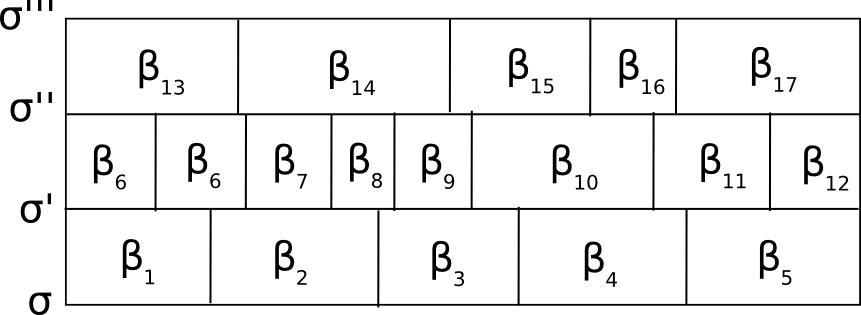
\includegraphics[width=200pt]{revert1.png}
\end{center}

Now, suppose that one of those blocks is invalid. Then, if we manage to revert immediately in the next block, the state will be moved to the red line here:

\begin{center}
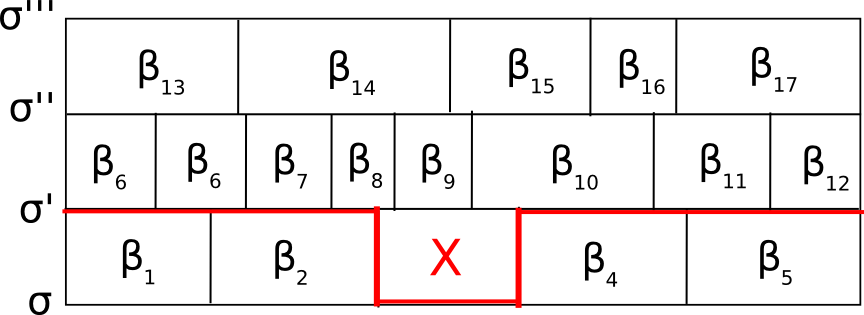
\includegraphics[width=200pt]{revert2.png}
\end{center}

And if we revert later, the state will be moved to the red line here:

\begin{center}
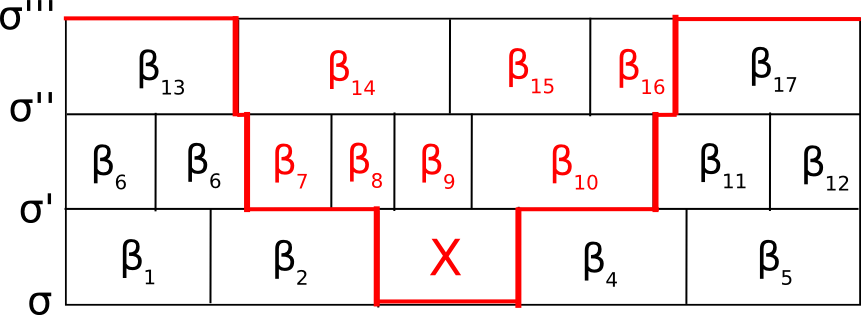
\includegraphics[width=200pt]{revert3.png}
\end{center}

Notice that one can apply the set of still-valid blocks sequentially to $\sigma$ to obtain $\sigma'_f$ in all cases.
\end{proof}

It is important to note that the revert process is scalable only if the number of substates that an attacker can revert with a single invalid block is bounded, assuming some bound on the amount of time that it takes for the bad block to be detected and for the revert to be included. Otherwise, the attacker can annoy all users by paying less than $b * L$ cost, and so the algorithm will no longer be scalable under attack. In order to achieve this, we have two solutions. First, we can specify that each block can have a maximum area size $k$ for some fixed $k$; the number of substates reverted assuming a revert after $l$ blocks will then be bounded above by $k^l$. The other approach is to require blocks with area larger than $k$ substates to have proportionately more validators; eg. a block with area of size $4k$ substates should require $\frac{8m}{3}$ signatures out of a pool of $4m$ in order to be valid. Both strategies ensure scalability under attack.

\chapter{Stacking}

The above schemes provide scalability up to $O(N^{2-\epsilon})$. But can we go higher than that? As it turns out, the answer is yes; we can in fact achieve scalability of $O(N^{d-\epsilon})$ for arbitrary $d$ while satisfying both economic and Byzantine-fault-tolerance guarantees. We accomplish this by essentially layering the scheme on top of itself. Essentially, we define a generalized transform $T(APPLY, VT, N, d)$ where $APPLY$ is a state transition function, $VT(F, s) \rightarrow F'$ is a function which takes a state transition function $F$ and a maximum header chain size $s$ and outputs the top-level state transition function $F'$ (eg. the algorithms we defined above can be seen as implementations of $VT$), $N$ is the maximum computational load and $d$ is the depth.

We define $T$ as follows:

\begin{itemize}
\item
$T(APPLY, VT, 2) = VT(APPLY, N^{1-\epsilon})$
\item
$T(APPLY, VT, d) = T(VT(APPLY, N^{d*(1-\epsilon)}), VT, d-1)$ for $d > 2$
\end{itemize}

We maintain the restriction that all objects produced at any point must have a soft maximum size, above which the number of validators required to agree on that object increases proportionately.

The definition is simple, and so somewhat obscures the complex inner workings of what is going on. Hence, let us provide an example. Consider a transform of the fallback-plus-subjective-resolution scheme provided above with $d = 3$. There would now be four ``levels'' of data structures. At the bottom level, we have the ultimate transactions that are affecting the state. Then, on the third level we have blocks containing those transactions. To validate blocks on this third level, there are $O(N^{2-\epsilon})$ validators (each with a deposit of size $O(N)$), which are recorded on the second level; a block on the third level must obtain signatures from $\frac{2m}{3}$ out of a pool of $m$ validators obtained from \emph{the entire pool} of second-level validators. However, the process of verifying that signatures from the correct validator pool are provided itself depends on data that is not shared globally (as it is on the second level), and so that process itself as a state transition function needs to be carried out using the two-level scalable protocol, ie. a second-level block would treat the second-level validators accessed by all third-level blocks contained inside of it as part of its ``observed area''. Blocks containing these transactions would themselves be voted on by the header chain, which has $O(N^{1-\epsilon})$ validators each with a deposit of size $O(N^2)$.

At this point, the algorithm almost has $O(N^{3-\epsilon})$ scalability, but not quite. To see why, note that each third-level block independently picks $m$ validators. Hence, if a second-level block has $O(N)$ transactions, and assuming that there are $O(N)$ second-level substates, we can expect a single second-level block to have an observed area of size $1 - \frac{1}{e^m}$ of the whole set of substates - which for even the absurdly unrealistic $m = 5$ amounts to almost all of it. Hence, there can be at most one second-level block, and so our scalability is right back to $O(N^{2-\epsilon})$.

To solve this problem, we make a moderate change: we say that the set of validators for any transactions should always be determined from the state \emph{at the start} of the super-block. Formally, we say that a superblock has two ``virtual transactions'' $\sigma -> (\sigma, \sigma)$ at the start, and then $(\sigma, \sigma') \rightarrow \sigma'$ at the end, and validators are selected from the left pool, not the right pool. This allows us to have validators be selected from anywhere in the state without including them into any observed areas. From an implementation perspective, this means that a block at any level would need to come with signatures $[s_1 ... s_m]$ and also Merkle proofs $[\pi_1 ... \pi_m]$ where $\pi_i$ proves that the validator $V_i$ that produced signature $s_i$ is indeed in the validator pool of the super-block's pre-state.

Now, consider the effort done at each level. In the header chain, we have $O(N^{1-\epsilon})$ validators, and each validator must on average perform top-level verification on $m$ blocks as before. On the second level, there would be $O(N^{2-\epsilon})$ validators, and there would be a total of $O(N^{2-\epsilon})$ blocks being produced, and so on average each validator would need to perform top-level verification on $m$ blocks. A second-level blockmaker would select an area $A$ of $k$ second-level substates, and fill the block with third-level blocks that have an effect inside that area; from the second-level validator's point of view, the third-level blocks look just like transactions would under an $O(N^{2-\epsilon})$ scheme, except with the difference that the validity condition requires verifying $m$ signatures. A third-level blockmaker would select an area of third-level substates, and fill the block with transactions that have an effect inside that area. Assuming the second-level blockmaker includes $O(N^{1-\epsilon})$ third-level blocks, and a third-level blockmaker includes $O(N^{1-\epsilon})$ transactions, all actors inside the system have less than $O(N)$ load.

Suppose that the scheme is attacked, by means of a successful invalid block at depth $d$. Then, a revert block would later be made on the same level, reverting the substate roots at that height, and the revert block would be processed just like a block. Because the total economic volume is $O(N^{k-\epsilon})$, and there are $O(N^{d-\epsilon})$ validators at depth $d$, the cost of bribing $m$ validators at depth $d$ would be $m * N^{d - k}$, and the block would inconvenience roughly $O(N^{d - k})$ users, so a proportionality of attacker cost to network cost is maintained. The same escalation argument as before shows that the scheme does not become unscalable until the attacker starts making economic sacrifices superlinear in the economic activity in the blockchain.

In practice, we expect that the extra complexity in implementing such an ultra-scalable scheme will be sufficiently high that cryptoeconomic state machine developers will stick to simpler two-level scaling models for some time. However, the result is important as it shows that, fundamentally, the level of overhead required in order to have a blockchain of size $L$ is roughly $m * log(L)$, a nearly constant value. With clever use of zk-SNARKs, a completely constant-overhead approach for blockchains of arbitrary size can almost certainly be achieved.

\chapter{Strategy}

The above sections described the \emph{algorithms} that can be used to convert a state transition function into validity criteria that can be used in order to build a scalable blockchain architecture out of traditional non-scalable components. However, there is also a need to develop higher-level \emph{strategies} that would be used by validators in order to allow a maximally expressive set of state transitions to effectively execute.

One major category of strategy that must be developed is for \emph{index selection}. Each block producer must determine what set of subspace indices they will be keeping up to date on the state for, and be willing to produce blocks containing. In the event that transactions requiring a larger area appear, the groups of block producers will likely need to somehow cooperate in order to be able to produce a block containing the combined area. One possible strategy is for validators to arrange subspace indices in a k-dimensional space, and maintain up-to-date knowledge of $\sigma[i]$ for either a radius-r cube or at least two adjacent subspaces. An alternative approach, specialized to simpler state transition functions involving sending from A to B (such as that of Bitcoin), is to maintain $(i, j)$ pairs and update $i$ and $j$ often. A third approach is adaptive: use some kind of algorithm to determine which subspace indices appear together most often, and try to keep track of an increasingly contiguous cluster over time. If transaction senders also adapt their activities to subspace boundaries, the co-adaptation process can potentially over time create highly efficient separations.

The other category of strategy is for transaction sending, particularly in the context of more complex state transition functions like that used in Ethereum. If a transaction only affects a few neighboring substates, then an index selection strategy as above will be able to provide easy and global transfer. However, what happens if an action needs to be performed that has wide-reaching effect, and it is impractical to put it into a single block? In this case, one option is to set up an ``asynchronous routing'' meta-protocol: if a transaction affects state $\sigma[i]$ but also needs to effect a change in $\sigma[j]$, then if it is acceptable for the latter change to be asynchronous we can have a message be passed through a ``network'' of contracts, first to a contract in a state neighboring $\sigma[i]$, then hopping progressively closer to $\sigma[j]$ during subsequent transaction executions until finally arriving at $\sigma[j]$ and effecting the desired change. Note that this is equivalent to the hypercubes \cite{hypercubes} strategy developed for Ethereum in 2014; but instead of being a core part of the protocol, the protocol has been abstracted even further out allowing hypercubes to simply be one of the many possible strategies that the protocol can lead to.

If the primary purpose of a blockchain is to act as a currency system, then as long as sufficient liquidity exists one can get by with a very low amount of interoperability. For example, even if it is only possible to move funds between substates every 1000 blocks, and even then only through a single central ``hub state'' (which is assumed all nodes store as a strategy), that limited movement provides enough fungibility for the currency units in the various substates to maintain fungibility. Cross-substate payments can be done by means of various decentralized exchange protocols, treating the different substates as different currencies with the only difference being that the currency exchange rate will always remain equal to 1. However, it is debatable whether this approach is preferable to the other strategy described above of having block proposers select random $(i, j)$ pairs.

Finally, there is the protocol-level decision of how to maintain the divisions between substates and grow and shrink the total number of substates if necessary. Adaptive algorithms, using strategies like Karger's minimal-cut algorithm \cite{karger}, may achieve optimal efficiency, but at the cost of sacrificing predictable gas pricing and thus imposing additional programming load on developers. An alternative approach is to simply create new substates every time the size of each substate increases beyond some value; ideally the target would grow with the square root of the number of substates, allowing the quantity of work at the second level and the quantity of work at the top level to grow in proportion to each other.

\chapter{Further optimizations}

The algorithms described above are meant to be starting points, and are by no means optimal. The primary areas of optimization are likely to be fourfold:

\begin{itemize}
\item
Reducing the limits imposed on state transition functions while maintaining identical levels of scalability
\item
Achieving constant-factor gains by increasing efficiency of Merkle proofs, block sending protocols, safely reducing the value of $m$, reducing churn, etc.
\item
Increasing block speed
\item
Making reverts less harmful by using inclusive blockchain protocols (ie. if $\beta_1 ... \beta_n$ is the set of blocks that was reverted, and $\sigma'_f$ is the post-revert state, automatically update to $\sigma''_f$ = $\sigma'_f {++} \beta_1 {++} ... {++} \beta_n$.
\item
Providing the option for even higher gains of efficiency but at the cost of less-than-perfect guarantees of atomicity, ie. reducing $m$ to $8$ with the associated cost gains but with the understanding that the action happens within a cordoned-off area of the state where invalid transitions will sometimes happen.
\end{itemize}

For the first of these, the most promising direction where one can find easy immediate gains is to try to separate observed area from affected area. Theoretically, there is no interference risk if two blocks in a super-block share observed areas, as long as that observed area is not any block's affected area. The challenge is (i) figuring out what hard limits to impose on a block in order to make sure that the scheme remains scalable (eg. if there are $\frac{n}{2}$ blocks each using $\{\frac{n}{2}+i\}$ as their affected area and $[\frac{n}{2}]$ as their observed area, the super-block will have $\frac{n^2}{4}$ hashes and will thus be unscalable), and (ii) figuring out how to manage reverts.

If one wants to go even further, one can allow the affected area of one block to be the observed area of another block, as long as one can arrange all blocks in an order such that each block is observed before it is affected. But there is a fundamental tradeoff between expressivity and fragility: the more the state transition function is able to process synchronous updates of very many and arbitrary states, the more costly a successful attack becomes if it must be reverted.

For the second, the largest tradeoff is likely to be that between churn and security. If one can keep the same $m$ nodes validating the same substates for a longer period of time, eg. half an hour, one may be able to reduce network load. However, keeping a constant pool for too long makes the scheme more attackable. Another option, particularly for schemes achieving hyper-quadratic scalability, is finding more effective ways of storing the set of validators so that it can be used without giving each mid-level block a large observed area (ie. we would like an area size $k$, not $k + m$).

For the third, the most likely source of gains will be improvements in the underlying non-scalable consensus algorithm used to maintain consensus on the top-level state $\psi$. Inclusive blockchain protocols such as those developed by Sompolinsky and Zohar \cite{inclusive} are a potential route for minimizing disruption under ultra-fast block times, and such protocols can also be used for the fourth goal of mitigating the impact of reverts.

For the fifth, an ideal goal would be to have a blockchain design which allows users to pick a point on the entire tradeoff space between cost and probability of failure, essentially capturing in the base protocol concepts like ``auditable computation'' \cite{auditable} (where computation is done by a third party by default, but if an auditor finds the third party provided an incorrect result the auditor can force the execution to be re-done on the blockchain and if the third party is indeed in the wrong it loses a security deposit from which the auditor will be able to claim a bounty).

Finally, there is plenty of room for optimization in strategies, figuring out how validators can self-organize in order to maximize the expressivity of the state transition function in practice. The ideal goal is to present an interface to developers that ``just works'', providing a set of highly robust abstractions that achieve strong security bounds, freeing developers of the need to think about the underlying architecture, math and economics of the platform unless absolutely necessary. But this problem can be solved much later than the others, and solutions can much more easily continue to be iterated even after the underlying blockchain protocol is developed.

\begin{thebibliography}{2}

\bibitem{mmpetertodd}
    Peter Todd on merge-mining, Dec 2013: \url{http://sourceforge.net/p/bitcoin/mailman/message/31796158/}

\bibitem{coiledcoin}
    What is the story behind the attack on CoiledCoin? (StackExchange, 2013): \url{http://bitcoin.stackexchange.com/questions/3472/what-is-the-story-behind-the-attack-on-coiledcoin}

\bibitem{parallelcomputing}
    Amdahl and Gustafson's laws and Bernstein's conditions for parallelizability (Wikipedia): \url{http://en.wikipedia.org/wiki/Parallel_computing#Amdahl.27s_law_and_Gustafson.27s_law}

\bibitem{zamfir}
    Vlad Zamfir's Formalizing Decentralized Consensus, coming soon.

\bibitem{merkle}
    Merkle trees (Wikipedia): \url{http://en.wikipedia.org/wiki/Merkle_tree}

\bibitem{zamfir}
    Vlad Zamfir and Pavel Kravchenko's Proof of Custody: \url{https://docs.google.com/document/d/1F81ulKEZFPIGNEVRsx0H1gl2YRtf0mUMsX011BzSjnY/edit}

\bibitem{ffterasurecode}
    $O(N*polylog(N))$ Reed-solomon erasure codes via fast Fourier transforms: \url{http://arxiv.org/pdf/0907.1788.pdf}

\bibitem{nxtinside}
    nxtinside.org, describing the NXT generation signature algorithm: \url{http://nxtinside.org/inside-a-proof-of-stake-cryptocurrency-2/}

\bibitem{snark}
    Succinct Zero-Knowledge for a von Neumann Architecture, Eli ben Sasson et al, Aug 2014: \url{https://eprint.iacr.org/2013/879.pdf}

\bibitem{schellingcoin}
    SchellingCoin: A Zero-Trust Universal Data Feed, Vitalik Buterin, Mar 2014: \url{https://blog.ethereum.org/2014/03/28/schellingcoin-a-minimal-trust-universal-data-feed/}

\bibitem{pepsilon}
    The P + Epsilon Attack, Vitalik Buterin, Jan 2015: \url{https://blog.ethereum.org/2015/01/28/p-epsilon-attack/}

\bibitem{sztorc}
    Truthcoin: Trustless, Decentralized, Censorship-Proof, Incentive-Compatible, Scalable Cryptocurrency Prediction Marketplace, Paul Sztorc, Aug 2014: \url{http://www.truthcoin.info/papers/truthcoin-whitepaper.pdf}

\bibitem{tendermint}
    Tendermint: Consensus without mining, Jae Kwon: \url{http://tendermint.com/docs/tendermint.pdf}

\bibitem{hypercubes}
    Scalability, Part 2: Hypercubes, Vitalik Buterin, October 2014: \url{http://www.reddit.com/r/ethereum/comments/2jvv5d/ethereum_blog_scalability_part_2_hypercubes/}

\bibitem{karger}
    Karger's minimal-cut algorithm, Wikipedia: \url{http://en.wikipedia.org/wiki/Karger%27s_algorithm}

\bibitem{auditable}
    Scalability, Part 1: Building on top, Vitalik Buterin, September 2014: \url{https://blog.ethereum.org/2014/09/17/scalability-part-1-building-top/}

\end{thebibliography}

\end{document}
